\documentclass{memoir}

\usepackage{import}
\import{../}{gov-style}
% \addbibresource{../thesis.bib}

\begin{document}
\epigraph{``Beep... beep... beep... beep...''}{\emph{Sputnik I}}
\section{Introduction}
\subsection{In space, no one will shoot you down}
Six flags rest on the surface of the moon: one fallen, five standing, and all American.\footnote{Well, they \emph{were} American. All of the flags are now bleached white after years of direct exposure to sunlight. (\cite{spudis_faded_2011})} Like the antarctic and the open seas, every nation may explore the moon, but none have the right to own it. Were China to launch a manned lunar mission tomorrow and plant its own flag on the surface, no one would question their right to do so, but no one would interpret that as a claim to ownership either. The history of human activity in space follows that exact pattern. A state has the unquestioned right to put anything in space, so long as it does not interfere with something that another state has already placed there. The Outer Space Treaty (OST), which entered into force only ten years after \emph{Sputnik}, formalized this practice: ``Outer space \textelp{} is not subject to national appropriation by claim of sovereignty, by means of use or occupation, or by any other means.''\footcite{noauthor_outer_1966} The strength of the OST has never been tested. Not once in the history of human space activity have hostile forces disabled, damaged, or destroyed an object in space that was not their own.

While it makes perfect sense that no state has attempted to enforce a territorial claim on the moon---technological feasibility aside, there's not much up there worth fighting for---artificial satellites present a more tempting target. Satellites are numerous, accessible, and undergird essential civil infrastructure. If a nation were so inclined, removing key satellites controlled by its adversaries could give them a significant strategic advantage. That an equilibrium held throughout the Cold War in which all satellites were left undisturbed---regardless of their applicability to military, commercial, or scientific ends---is one of the most remarkable achievements of \nth{20} century diplomacy. The world today relies on communication infrastructure that only exists because the safety of the satellites that make it possible is functionally guaranteed by decades of peace in outer space.

At the dawn of the space age, the safety of artificial satellites was far from guaranteed. Four years after the first U-2 overflight, a familiar dynamic could have played out when the first spy satellite launched in August 1960: the US develops a new photo-reconnaissance technology which its main adversary is unable to prevent; the USSR diplomatically objects to the technology's use; the USSR finally develops a weapon capable of counteracting the new technology; and the USSR employs it. Each one of these steps came to pass except the last---even after developing a feasible anti-satellite (ASAT) weapon, the Soviet Union never made use of it. And the onus was on the Soviets to push back against American efforts to normalize satellite reconnaissance. \emph{Sputnik} briefly put the USSR at the forefront of the final frontier, but the satellite itself was totally innocuous; it obtained data about the density of the atmosphere and propagation of radio waves.\footcite{nasa_sputnik_2019} It was the United States that would first launch a satellite capable of photo-reconnaissance---and it was the Soviet Union that allowed it to happen.

Spy satellites are not just one of the best edge cases for norm against shooting down a satellite, they are the reason it exists in the first place.\footnote{I'm not suggesting that, absent spy satellites, nations would have just constantly shot down each other's weather satellites. But remember that the CIA planned a cover for the U-2 in which it was a ``weather plane'' that had gone off course. The USSR forced a cargo plane to land in Hungary because they suspected it of espionage. That never happens in space, because intelligence norms are strong enough that the accusation of dual-use is never even raised. There are no good and bad satellites; as long as a satellite doesn't have literal weapons, then there is no plausible reason to shoot it down.} The reconnaissance satellite succeeded because the Eisenhower administration purposefully designed its space program to establish a norm of peaceful development in space---with the single goal of legitimizing satellites for intelligence-gathering. As a result, the United States finally gained unrestricted access to aerial intelligence of the type that an Open Skies policy might have provided. That all satellites, regardless of purpose, are immune to hostilities as a result is just a happy byproduct.

In this chapter I will explain how the United States developed a norm protecting the use of reconnaissance satellites, and how that norm continues to prevent the use of ASAT weapons today. Unlike in previous chapters, it is not necessary to prove that there is a muted diplomatic response to satellite espionage because the lack of response is self-evident: no military action has ever been taken against satellites, and the Soviet Union only objected to reconnaissance satellites until it were able to make its own. The first section looks at the 10-year period prior to the first spy satellite, during which the United States began to build a diplomatic strategy that would legitimize its eventual launch. The following section analyzes the deployment of early spy satellites, and how they altered the security dynamic between both the US and the USSR. The final section looks at threats to the norm, from the Reagan era to the present today.

\section{Framing the spy satellite}
\subsection{Planning for a new security environment}
The successful launch of a spy satellite in August 1960 was the culmination of a decade-long grand strategy to neutralize the Soviet Union's greatest military advantage, and secure the United States against a surprise nuclear attack. Though the US air-atomic capabilities in the early Cold War discouraged the USSR from making more use of its conventional military advantage, the USSR quickly developed nuclear weapons of its own and was rapidly developing longer-ranged delivery systems. The fear of a surprise nuclear attack haunted Eisenhower throughout his presidency.\footcite[p.~68]{killian_sputnik_1977} American status and security relied on the ability to accurately asses Soviet capabilities and foresee such an attack, and producing those accurate assessments required state-of-the-art intelligence.

As detailed in previous chapters, the closed nature of the Soviet state posed a significant challenge to American intelligence efforts. One of the Eisenhower administration's highest priority foreign policy goals was to permanently rectify this imbalance by opening up the Soviet state to photo-reconnaissance.\footcite[p.~65]{hayes_struggling_1994} With little information emerging from the USSR of its own volition, and the difficulty of running human agents deep within a paranoid surveillance state, some novel technical approaches would be required. Spy planes, artificial satellites, and other then-futuristic reconnaissance possibilities had been discussed since the end of WWII, but they remained theoretical concepts for many years. That all changed in 1954, when Eisenhower met with the Office of Defense Mobilization's Science Advisory Committee, and requested that it put together a task force which would tackle the problem of America's vulnerability to a surprise attack.\footcite[p.~67. The president's science advisor described this moment as the starting point for ``any complete account of how science advice was mobilized for the use of President Eisenhower.'']{killian_sputnik_1977}

Chaired by MIT President Dr. James Killian, the Technological Capabilities Panel (TCP) was tasked with forecasting America's strategic position and presenting possible technical solutions to mitigate the threat of a nuclear Pearl Harbor.\footcite[p.~115]{mcdougall_heavens_1985} The panel presented its results in February 1955---a report formally titled ``Meeting the Threat of a Surprise Attack,'' but also variously referred to as the ``Killian Report,'' ``TCP Report,'' or ``Surprise Attack Study.'' The report predicted four distinct periods of relative power would unfold over the next decade, starting with the current era, in which the US had a relative advantage in air-atomic power but was not capable of a decisive strike, and ending in a world where mutual ICBM capabilities ensured that the balance of power would remain a stalemate indefinitely.\footcite[p.~116]{mcdougall_heavens_1985}

All four Cold War phases that the Killian Report predicted---with shocking accuracy, as it turned out---had one thing in common: the sobering calculation that a great power conflict would result in heavy American losses. Even in the phase where the balance of power most favored the Americans (before the development of Soviet multimegaton capability), the United States ``would be severely damaged,'' and ``emerge a battered victor'' in the event of a surprise attack.\footcite{technological_capabilities_panel_meeting_1955} Killian wrote that, while presenting the report to the National Security Council (NSC), ``we emphasized that even though our \emph{relative} military strength might change in the manner suggested in the table, we still would be in a position where the United States could be grievously hurt.''\footcite[p.~75]{killian_sputnik_1977}

Therefore it was of paramount importance to avoid a general conflict at all costs, and the report was split into different subgroups that approached the problem from all angles. One subgroup, for instance, analyzed the progress of the ICBM program; building more missiles and more advanced missiles remained central to American deterrence policy throughout the Cold War. But not all of the subgroups were focused on offensive capabilities; another subgroup devoted themselves to studying novel approaches for intelligence-gathering. ``We \emph{must} find ways to increase the number of hard facts upon which our intelligence estimates are based,'' the Intelligence Section states, ``to provide better strategic warning, to minimize surprise in the kind of attack, and to reduce the danger of gross overestimation or gross underestimation of the threat.''\footcite{technological_capabilities_panel_meeting_1955} The entire security position of the United States relied on the country developing scientific means to minimize the risk of miscalculation.

\subsection{The spy plane walked so the spy satellite could run}
One of the TCP recommendations was the subject of the previous chapter. The panel learned that the Air Force had rejected a proposal from Lockheed for a long-range, jet-powered glider. The scientists in charge of the Intelligence Section---led by Edwin Land, co-founder of Polaroid---realized that when equipped with photographic equipment and other intelligence devices, the Lockheed prototype had the potential to serve as a revolutionary information-gathering machine.\footcite[p.~81-82]{killian_sputnik_1977} They proposed that Eisenhower approve what came to be known as Project Aquatone; the president accepted; and development of the U-2 spy plane began. At the same time, the Eisenhower's positive reaction to the Killian Report caused both the CIA and the Air Force to accelerate their existence plans for reconnaissance satellites.\footcite[p.~83]{killian_sputnik_1977}

The U-2 revolutionized aerial reconnaissance, but even in the early days when it remained literally untouchable, the intelligence that it provided had limitations. While the U-2 provided CIA imagery analysts with impossibly high-resolution photos of an individual military base, it was less helpful in determining the locations of various military bases throughout the vast expanse of Soviet territory. Eisenhower was never going to order 30 U-2 planes to fly over the Soviet Union at once---that would have looked like an invasion---but he could orbit the same satellite 30 times around the Earth, photographing a slightly different section of the USSR each time, and building a comprehensive picture of their military installations.\footnote{Here's how this works. The \emph{Discoverer} satellites that I discuss in this chapter were launched into a ``polar orbit,'' meaning they passed over polar regions. In the time it takes the satellite to complete a full orbit, the Earth has rotated slightly underneath it, so the satellite photographs an area that is longitudinally shifted each pass. Think of a winding a piece of string around a ball with your right hand, while slowly rotating the ball with your left. I mention this because, in addition to being incredibly interesting, the physics actually have an enormous effect on how the satellite is received. Each one is performing a whole series of overflights; but from a psychological perspective, it's one missile launch, one satellite, one overflight. Though outside the scope of this thesis, it would be worthwhile to explore how technological advancements can create a psychological distinction between strategically identical acts, or as is the case here, make the vastly more threatening act seem like the one that is less so.} The spy plane offered depth; the spy satellite promised breadth. Together, they could operate for complementary purposes: a spy plane dispatched when high quality localized intelligence was required, and a satellite to form a more comprehensive picture of the Soviet military posture. And of course, satellites could deployed to surveil dangerous territory without risking the life of a pilot.

The breadth of information that a satellite could provide might also dispel the Eisenhower administration's political albatross---his supposedly dovish defense spending. Eisnhower faced constant pressure to increase the defense budget and close the alleged ``missile gap'' between the US and the USSR. While U-2 photography (codenamed ``Talent'') had been helpful for pushing back against these demands, the diplomatic volatility of each flight limited the amount of ground that it could cover. In July 1960, the CIA's Photographic Interpretation Center conducted a study to determine how much of the Soviet territory that it deemed suitable for ICBM deployment had been observed by Talent photography since January 1959. As it turned out, very little. The ``intelligence bonanza'' from Aquatone had still only observed roughly 13.6\% of the viable Soviet terrain. Visual observations from other sources added an additional 1.5\%.\footcite[A significant portion of this document is redacted, including, for some reason, the page numbers.]{cia_future_1960} Satellites showed enormous potential for covering that remaining 85\%, and in doing so, shut down discussion of the ``missile gap'' once and for all.

Even more important than the the technical benefits of a spy satellite were the potential political ones. Because the territorial boundary conditions of outer space were completely undefined, the spy satellite might able to perform photo-reconnaissance overflights with a consistency that a spy plane never could. When the U-2 started flying missions in 1956, it flew high enough to avoid Soviet anti-aircraft capabilities, but that status quo had a clear expiration date. The overflight program was so risky that it was originally intended to last only a year or two.\footcite[p.~33]{lindgren_trust_2000} The Soviets considered overflights to be a violation of their territorial sovereignty, and continued to register diplomatic protests about them. Satellites, by contrast, operated in a new space that had the potential to transcend airspace norms, where they could fly ``over'' Soviet territory with impunity. Historian Walter McDougall aptly summarizes the promise of spy satellites in his book on the political history of the space age:

\begin{quote}
	If continuous surveillance of Soviet installations and exact targeting of Soviet bases were to be assured, the solution was to spy from outer space. Camera-toting satellites, circling the earth south to north [sic] in a polar orbit, could view the entire surface of the earth as it rotated below, return to any location in a few days' time, hone in on suspicious areas, and do it all under the legal cover of freedom of space---if such legal cover could be established. Given the simultaneous USAF go-ahead for Project WS-117L and Land's insistence on applying the most advanced knowledge of science and technology to intelligence, there is little doubt that the portions of the Killian Report that remain classified to this day include the recommendation that the highest national priority attach to the development and operation of reconnaissance satellites.\footcite[p.~117]{mcdougall_heavens_1985}
\end{quote}
The key phrase here is ``if such a legal cover could be established.'' The undefined legal status of space presented an opportunity, but also a challenge. The TCP understood that the Soviet Union would likely recognize the enormous advantage that a spy satellite would confer on the US, and object to their deployment using any international norms possible.  It was therefore necessary to present reconnaissance satellites in such a way that would limit the grounds for objection. Fortunately, plans for that were already underway, and the TCP found them.

Though the Killian Report first elevated the issue to a top national security priority, American policymakers had been considering how to politically frame the space program for years. The Air Force commissioned a series of studies about the potential for artificial satellites from 1946 to 1947, and concluded that they were feasible, but not necessarily practical.\footcite[p.~5-6]{peebles_corona_1997} Progress was limited until 1950, when  the Air Force again commissioned the RAND corporation to study the potential military utility of artificial satellites. The resulting report, according to McDougall, ``deserves to be considered the birth certificate of American space policy.''\footcite[p.~108]{mcdougall_heavens_1985} By my accounting, ``The Satellite Rocket Vehicle: Political and Psychological Problems'' should also be considered the birth certificate of American strategic intelligence policy---and the international norms that resulted.

The RAND report succinctly presented the challenges that intelligence norms faced at the outset of the Cold War, and the benefits that the US stood to gain by promoting them. The potential damage that spy satellites posed to the Soviet strategic posture was considerable, and the Soviet Union, politically and culturally, was singularly sensitive to invasions of privacy. ``Fear of loss of secrecy is constant and intense,'' the report noted, and ``it is to be expected that attacks upon secrecy will be construed as attacks upon Soviet sovereignty.''\footcite[p.~14]{kecskemetic_satellite_1950} It concluded that the USSR would likely see a novel reconnaissance satellite as a major threat, altering the balance of power between the two states, and take the appropriate measures to counteract it.\footcite[p.~13]{kecskemetic_satellite_1950}

The report also made clear that, even before developing ASAT capabilities, the USSR would have plenty of options to put pressure on the United States that fell short of total war. They might pursue litigation in the International Criminal Court, the outcome of which would be uncertain, especially if there were evidence that the satellite was gathering intelligence.\footcite[p.~16]{kecskemetic_satellite_1950} Or, if the satellite required receiving stations in foreign countries, the USSR could put pressure on the host countries to shut the stations down, threaten to destroy the stations, or simply attack the stations with military force.\footcite[p.~16-17. Importantly, these are all things that the Soviet Union could also have done with the U-2 spy plane. In fact, they might have even been more effective. Unlike the U-2 planes that took off from allied airfields, the first spy satellite, Project Corona, ejected a film capsule and required no such receiving stations. The US was somewhat more circumspect with its overflights, but the options were there.]{kecskemetic_satellite_1950}

These results sparked a renewed Air Force interest in reconnaissance satellites, and the service began putting together the hardware specifications for one in 1951. These specifications became Project WS-117L, ``a strategic satellite system,'' and the first American space program.\footcite[p.~110-111. The WS is short for ``Weapons System.'']{mcdougall_heavens_1985} When the members of the TCP began to survey the possibilities for the future of American strategic reconnaissance, they found Project WS-117L, exactly the kind of technical innovation that they were looking for.\footcite[p.~197]{brugioni_eyes_2010} But the United States could not begin the space age with a spy satellite. Doing so would ensure that outer space became yet another arena for conflict, the way airspace had at the turn of the \nth{20} century. What happened instead reflects incredible forethought on the part of Eisenhower and his administration, who baked intelligence norms into the legal framework of outer space, then launched a spy satellite into the legal regime that they created.

\subsection{Spiking the space race}
Everything about the administration's space policy was carefully crafted to set the stage for the eventual launch of a spy satellite. From the time that artificial satellites first appeared viable until he left office, Eisenhower used the civilian space program as a public means of diverting attention from the security-related programs he valued.\footcite[p.~119]{day_eye_2015} Acting on the recommendations of the TCP, the National Security Council (NSC) proposed a scientific satellite program in May 1955, which Eisenhower accepted. In this memo, NSC-5520, the NSC Planning Board argued that, when framed properly, a scientific satellite could be used as diplomatic tool to promote a norm establishing ``freedom of space.'' The proposal tracks closely with a similar one from the 1950 RAND report, which suggested that the US first launch an innocuous ``experimental satellite'' that did not cross over Russian territory, and gauge the diplomatic reaction.\footcite[p.~21]{kecskemetic_satellite_1950} The political framing of the satellite is discussed at the top of NSC-5520, in a section entitled \emph{General Considerations} (emphasis mine):

\begin{quote}
	6. \textelp{} \textbf{Furthermore, a small scientific satellite will provide a test of the principle of “Freedom of Space”. The implications of this principle are being studied within the Executive Branch.} However, preliminary studies indicate that there is no obstacle under international law to the launching of such a satellite.

	7. \textbf{It should be emphasized that a satellite would constitute no active military offensive threat to any country over which it might pass.} Although a large satellite might conceivably serve to launch a guided missile at a ground target, it will always be a poor choice for the purpose. A bomb could not be dropped from a satellite on a target below, because anything dropped from a satellite would simply continue alongside in the orbit. \footcite{nsc_planning_board_draft_1955}
\end{quote}
Even though there was no international law prohibiting the use of satellites, a theoretical ``freedom of space'' principle depended on the first satellite not having military purposes. What NSC-5520 did not anticipate was that the US wouldn't have to establish that principle on their own. On October 4, 1957, the Soviet Union launched the world's first artificial satellite, a small metal ball named \emph{Sputnik}.

Getting beaten to orbit by \emph{Sputnik} put the United States at an advantage. The Soviets could hardly denounce the American satellite program as suspicious when they very publicly made the first move---and without asking permission to orbit over the United States.\footcite[p.~40]{peebles_corona_1997} The US didn't \emph{try} to lose first leg of the space race, per se, but policymakers were aware well in advance that being second to launch a satellite had its advantages. Reviewing NSC-5520, Nelson Rockefeller wrote that since the Soviets had already announced plans to launch a satellite, the existence of their project could be used to good effect against the inevitable Soviet protests about the American satellite program.\footcite[p.~120]{mcdougall_heavens_1985} Though ideally the US would be able to set the precedent for ``freedom of space'' itself, senior administration officials understood that if the USSR launched first, then the American satellite program would be almost automatically justified.

Not only did the Eisenhower administration understand that being second to orbit came with a significant consolation prize, they were not particularly focused on winning the space race to begin with. Launching the first satellite was assigned the lowest possible priority because the administration correctly determined that their other goals---finishing the ICBM, monitoring Soviet R\&D, and framing the satellite program as a civilian scientific endeavor---were of greater strategic importance in the long term.\footcite[p.~123-124]{mcdougall_heavens_1985} Eisenhower himself repeatedly dismissed concerns about the prestige of being the first nation to orbit an object in space, openly contemptuous to the idea that space was any kind of race at all.\footcite[p.~100]{lindgren_trust_2000} His complete disdain for what he called ``stunts'' would prove to be disastrous politically, but from the standpoint of international law, his restraint was crucial to establishing a strategically beneficial precedent.\footcite[p.~134]{day_eye_2015}

In fact, the overriding American priority to legitimize reconnaissance satellites is probably the \emph{reason} that the Soviets started the Space Age instead. Just as Eisenhower limited the involvement of the Air Force in Aquatone to paint the U-2 as a civilian project, he made technical decisions that were intended to make the scientific satellite seem as non-threatening as possible, and none was more important than the vehicle that would launch it. The group tasked with implementing NSC-5520 had to choose between competing launch proposals from the Army, Navy, and Air Force. It made the somewhat surprising choice to go with the unproven Navy Research Laboratory (NRL) \emph{Vanguard} rocket, even though the Army Ballistic Missile Agency (ABMA) engineers, headed by famous rocketeer Wernher von Braun, had been developing their proposal for a year. Among the reasons the committee gave for their decision, two stand out. First, the NRL impressed the committee with its plans for scientific components and a radio tracking system.\footcite[p.~122]{mcdougall_heavens_1985} Second, the panel purposefully wanted to avoid using a ballistic missile to launch a scientific satellite.\footcite[p.~129. Though the NRL is run by the Navy, it functions like a civilian scientific operation. Everything that I have read about this decision seems to take it for granted that despite the Navy involement, the NRL proposal would be seen as a civilian project. This makes sense to me, especially when you consider that it was competiting with the same agency that was building nuclear delivery systems.]{day_eye_2015}

Launching the first satellite with a ballistic missile threatened to compromise both of the principal national security priorities. It might delay the development of the ICBM, which posed an existential threat to American military superiority, and it would jeopardize the civilian character of the satellite program, which the committee members knew was necessary to establish ``freedom of space.''\footcite[p.~122]{mcdougall_heavens_1985} The Von Braun engineers vigorously protested the decision, because they believed---correctly---that their proposal would succeed first. But being first in space was not the goal, establishing a legal precedent was. Von Braun's appeals were continually rejected, and always for the same reason: launching a satellite with no scientific purpose other than demonstrating superiority would compromise the moral high ground which the US desperately needed to secure.\footcite[p.~131]{day_eye_2015}

Publicly, \emph{Vanguard} was a disaster. The rocket experienced an embarrassing setback on December 6, 1957, when it failed to launch a three-and-a-half pound satellite, just after the USSR had successfully launched \emph{Sputnik II}.\footcite[p.~119]{killian_sputnik_1977} The Soviets had put a dog in space before the Americans even managed to get a satellite up there.\footcite[Her name was Laika.]{george_sad_2018} When then United States finally succeeded in launching at satellite, it was not thanks to the \emph{Vanguard}, but rather the ABMA team that had been consistently rebuffed by the administration. Finally given the chance, Von Braun and his engineers quickly accomplished what they had always said they would: modify a Jupiter-C ballistic missile to send a satellite into orbit. The Army launched \emph{Explorer 1} on January 31, and it carried a pioneering array of miniaturized electronics, including two micrometeoroid detectors and a Geiger counter.\footcite[p.~168]{mcdougall_heavens_1985} \emph{Explorer 1} and \emph{Vanguard 1}, which launched about six weeks later, provided an impressive amount of scientific data in comparison to the Sputniks.\footcite[p.~168]{mcdougall_heavens_1985} More importantly, even though the US did end up launching their first satellite using a ballistic missile, its visible defeat in the space race and clear scientific purpose had the intended effect of blunting Soviet efforts to characterize the American satellite program as a military development. It was time to launch a spy satellite.

\section{How Corona changed the Cold War}
\subsection{The blackest of black projects}
The Soviet Union unintentionally set an early precedent for ``freedom of space,'' but that did not automatically justify using space for reconnaissance. As far as the international community was concerned, it had only been established that overflights were permissible for scientific purposes; military reconnaissance was still an open question.\footcite[p.~47-48]{peebles_corona_1997} Now that the space age was underway, successfully normalizing photographic satellite overflights was the next step, and it required tight message discipline across all levels of government. Unfortunately, information about WS-117L, the Air Force reconnaissance satellite program, had already begun to leak.\footcite[p.~96]{lindgren_trust_2000}

Like many of Eisenhower's decisions on space policy, the plan he came up with was a brilliant long-term success---but a complete mystery to the public and utterly baffling to most of the military establishment. Originally, WS-117L was intended to be a family of reconnaissance satellites. Eisenhower simply selected the most immediately promising project---a single-use film-retrieval satellite, codenamed Corona---and canceled it. Air Force personnel were ``thunderstruck.''\footcite[p.~45]{peebles_corona_1997} With public bewilderment instilled and American reconnaissance satellites now seemingly a few years out, the administration began a multi-pronged approach to legitimizing spy satellites. Publicly, the US government advocated for a ``freedom of space'' policy that explicitly included reconnaissance like the WS-117L project, and, quietly, it resurrected the Corona project under deep-cover CIA administration.

The first part of this strategy required international approval for space-based overflights, and the US suggested that the United Nations create the UN Ad Hoc Committee on the Peaceful Uses of Outer Space (COPUOUS) to deal with precisely this issue. The Soviets, worried about having the limitations of their ICBM program exposed, refused to participate for years.\footcite[p.~140]{day_eye_2015} Meanwhile, the actual spy satellite program progressed at an accelerated pace, and with unmatched secrecy. The team started with only 30 personnel and eventually swelled to 300, almost none of whom knew the entire scope of the project. Team members had to take different routes to work to avoid being followed and were never allowed to say the word ``Corona'' on the telephone, or even the abbreviation ``C.''\footcite[p.~51]{peebles_shadow_2000} As far as the government was concerned, Corona's cover was bulletproof. When the satellite began making test launches, the US heavily promoted its new \emph{Discoverer} program as a scientific achievement---confident that its status as a front for the Corona project could not be proven false the way the U-2's cover had been just three months prior. When it finally succeeded in recovering a \emph{Discoverer} satellite from orbit, the US government released photographs of the first successful capsule triumphantly floating in the water, and an American flag retrieved from within was presented to the president.\footcite[p.~83]{peebles_shadow_2000}

Today's Earth-imaging satellites have enormous solar panels, radio their images down to command stations, and have mission durations in a scale of years. \footnote{This design simply did not work with film. A rival project that developed the film midair and transmitted the data back down failed to provide intelligence of sufficient quality. (\cite[p.~203-204]{brugioni_eyes_2010}) The last film-based orbiting reconnaissance camera developed for the U.S. Government was the KH-9 HEXAGON, which operated between 1971 and 1986. It was famously complicated, with four separate film-reentry pods (\cite{pressel_spy_2013}). I presume the rest since then have been digital, but because the HEXAGON was only declassified in September 2011, it will likely be quite a long time before we find out.} Corona was nothing like that. Instead, each satellite was little more than a monstrously expensive disposable camera. The plan for a Corona flight looked like this: the satellite would be sent into space carrying enough film for a 24-hour mission, and its camera would switch on every time the satellite flew over denied territory. After completing seventeen orbits, the satellite would pitch down 60 degrees and eject the film capsule back down to Earth. Various rocket systems would stabilize it, a heat shield would protect it, and a series of parachutes would decelerate it. What remained of the capsule would hopefully descend within a 200-by-60 mile recovery zone (``the ballpark''), but at the very least within the boundaries of an additional 400-mile section (``the outfield''). Ideally, it would be caught in midair by a cargo plane.\footcite[p.~56]{peebles_corona_1997}

Why is that significant? Because at no point was satellite reconnaissance a \emph{fait accompli}---each launch was another opportunity for the Soviet Union to object to the continued use of a potentially illegal surveillance method. And there were a great many launches. From February to August 1960, right in the middle of the U-2 incident, twelve test launches failed before the US achieved the first successful recovery of a Corona satellite---of any object from orbit in the human history, for that matter---when it fished \emph{Discoverer 13} out of the sea. The US repeated that feat with \emph{Discoverer 14} a week later, and this time it carried a camera, bringing invaluable intelligence back from space that dealt a mortal blow to the myth of the missile gap.\footcite[p.~101-102. The previous failures had been so demoralizing that \emph{Discoverer 13} only carried diagnostic equipment, which made its success all the more exciting. Ships on standby were able to retrieve the satellite even though it fell outside the recovery zone---\emph{Discoverer 13} many not have landed in the ballpark or the outfield, but in many respects, the mission was a home run.]{lindgren_trust_2000} The launches kept coming---the next one to return high quality photos was \emph{Discoverer 18} in December. Eisenhower left office soon after, but between \emph{Discoverer 18} and \emph{Discoverer 38}, twenty launches were performed, two of which carried actual radiometry equipment (in support of Corona's cover story), and seven produced film of high enough quality for the mission to be considered a complete success.\footcite[p.~103]{lindgren_trust_2000}

Like the U-2 overflights, this intricate process was immediately identified by the Soviets for what it was: a military reconnaissance effort. The Soviet Union protested the very first \emph{Discoverer} launch, correctly alleging its military purpose even though the satellite had failed, and would fail eleven more times.\footcite[p.~140]{day_eye_2015} Until 1963, Soviet propaganda continually railed against the Americans, in domestic media and international forums, for attempting to militarize space.\footcite[p.~271]{mcdougall_heavens_1985} The USSR sponsored a UN resolution to prohibit espionage from space, and Khrushchev vowed that his military would shoot down spy satellites, just as they had the U-2.\footcite[p.~166]{day_eye_2015} In the first few years after the United States developed satellite reconnaissance capability, it appeared that the USSR was acting exactly as the 1950 RAND report had predicted, and using every legal means at their disposal to end the satellite overflights.

\subsection{The effect of Corona photography on Soviet security}

Khrushchev had every incentive to discourage satellite reconnaissance, because the intelligence that the US gained through Corona was absolutely devastating to Soviet claims about their military prowess. The U-2 overflights had sufficiently debunked the ``bomber gap,'' and seemed to suggest that no ``missile gap'' existed either.\footcite{goodpaster_cold_2003} But as the CIA report on Talent photography showed, being unable to find ICBM sites was not conclusive proof that they did not exist, and the vast majority of possible missile sites remained un-photographed. Confusion about Soviet long-range attack capabilities still existed at various levels of government, confusion which ultimately led to the doomed flight of Gary Powers.\footcite[p.~344]{brugioni_eyes_2010} It was the \emph{Discoverer 14} and \emph{Discoverer 18} missions that successfully photographed the sites that intelligence analysts considered most likely to host operational ICBMs, and found nothing.\footcite[p.~379]{brugioni_eyes_2010}

To make matters worse for the Soviets, the moment at which the US discovered that the USSR had far fewer missiles than they claimed was the exact moment at which that disparity was greatest. The missile gap actually went in the other direction---in 1962, the US had more than double the ICBMs, maintained a substantial lead in manned bombers, and had just begun to deploy nuclear submarines.\footcite[p.~251]{mcdougall_heavens_1985} By the time of the 1960 presidential election, both sides of the Cold War had a generally accurate read on each others' military capabilities, and they knew that their adversary was properly appraised of the strategic situation as well.  If Khrushchev genuinely feared an American attack, absolutely nothing would have been a greater threat to Soviet security than the collapse of the USSR's most significant deterrent argument.

Not only did Corona make a theoretical offensive attack more likely, it made the plans for such an attack significantly more effective. The impact of the project on military planning is best summarized by how it affected the joint American-British plan for an offensive against the Soviet Union, which aerospace historian Curtis Peebles describes here:

\begin{quote}
Starting in 1962, the Corona photos were also used for nuclear targeting. Corona photos provided the first accurate coordinates of Soviet military facilities. This resulted in a shift in U.S. policy. During the 1950s, little was known about the location of Soviet military bases. The lack of information was reflect in the first join SAC-RAF Bomber Command strike plan. The plan, which went into effect on October 1, 1958, assigned 106 Soviet targets to the RAF bomber force: 69 cities, 17 airfields, and 20 air defense targets. A full two-thirds of the targets were cities. This disparity was ever greater with the unilateral RAF strike plan. If Great Britain should be forced to attack alone, ninety-eight Soviet cities would be bombed.

On August 1, 1962, a revised joint plan went into effect. The changes, which reflected a full two years of Corona operations, were profound. The RAF Thor IRBMs and bomber force would strike forty-four ``offensive capability'' targets such as airfields, ten ``defensive capability'' targets such as air defense control centers, twenty-eight Soviet IRBMs sites, and only sixteen cities. Urban targets had gone from the majority to next to last in number. The unilateral British plan also underwent a similar change.\footcite[p.~139]{peebles_corona_1997}
\end{quote}
The Soviet Union lost its most significant military advantage over the West in a little under two years. No subsequent missile buildup or bunker hardening or second-strike capability could undo the damage done to the Soviet military posture when \emph{Discoverer XIV} and its successors sailed past the Iron Curtain. And yet the only thing the Soviet Union did in response was publicly protest the spy satellites, and refuse to accept American proposals for a legal regime that included the rights of reconnaissance overflights. Those protests continued for about 3 years, until the Soviets developed their own working spy satellites, ``freedom of space'' became a mutually-agreeable reality.\footcite[p.~271-275]{mcdougall_heavens_1985}

\subsection{The final normalization of spy satellites}
From the perspective of the United States, it seems obvious that the Soviet Union had almost everything to lose by legitimizing the use of spy satellites. Aerial reconnaissance neutralized one of Soviet Union's asymmetric structural advantages---the inherent secrecy of Soviet society---and put a dent in their claims to an arms advantage too. What it gained in return is tough to say, but there is no possibility that it matched the intelligence windfall that befell the CIA. Aerial reconnaissance was the top national security priority of the United States during the Eisenhower administration. Their legitimization of spy satellites dealt an indisputable blow to Soviet standing. So why did the Soviet Union let it happen?

The brilliance of the American strategy goes a long way towards explaining why the USSR ultimately allowed satellites to fly over its territory. Both the overt and covert halves of the strategy played an important role. If the US had not been engaging in multinational talks about science and the freedom of space at the same time it was launching spy satellites, then it is very likely that upon developing ASAT capabilities, the USSR would have simply started shooting them down. That would have been an almost identical situation to the U-2 saga, and it was essential that when ASATs became available, the USSR not presume to have the unquestioned right to use them.

But if the US had not been simultaneously running a covert program before the norm was established, then how would the norm have ever been established at all? At what point would the United States have determined that it was officially legal to launch a spy satellite? Soviet intransigence on COPOUS demonstrated that they were unwilling to formally acknowledge the use of spy satellites, so no legal solution was forthcoming. The Soviet Union was also unlikely to launch the first spy satellite; its HUMINT operations were able to provide most of the intelligence that a photo-reconnaissance operation would have provided and launching the first spy satellite would give Americans the perfect excuse to close the intelligence gap once and for all. The situation that resulted was a perfect storm for the normalization of satellite reconnaissance: the Soviet leadership found that they had the ability to develop a reliable spy satellite much sooner than they could develop a reliable anti-satellite weapon, of which their right to use would still be uncertain. The path of least resistance, but greatest preservation of pride, was to simply start spying themselves.

A few Khrushchev own-goals played a part in legitimizing satellite reconnaissance as well. At the infamous four-powers summit in 1960, after watching Khrushchev vent about the U-2 Incident, French president Charles de Gaulle calmly told him: ``You're making too big a fuss about the matter. There is probably a ton of Russian iron [referring to Russian satellites] coming through French space every day without my permissions. I have no idea what is inside those satellites and you have not told me. But I am not making a big fuss.'' Khrushchev admitted that the Soviets had put cameras in some satellites, but not necessarily any that flew over France.\footcite[p.~353]{brugioni_eyes_2010} He went on to say that he only considered airplanes to be out of bounds, not satellites. In Eisenhower's later paraphrasing, Khrushchev said that ``any nation in the world who wanted to photograph the Soviet areas by satellite was completely free to do so.''\footnote{PUT EISENHOWER BOOK HERE.} Even being the first nation to space played a role. Of course, it cannot be said that launching the first satellite in human history was a \emph{mistake} on the part of Khrushchev---Eisenhower underestimated the symbolic importance of igniting the Space Age, to his significant political detriment---but it is indisputable that \emph{Sputnik} made it much harder for the USSR to argue that reconnaissance satellites were an imperialist invasion of territorial sovereignty.

And yet, American strategy and Khrushchev's missteps still do not fully explain why Soviet Union continued to permit photo-reconnaissance after ASATs were developed. The weapons were feasible; the USSR started testing its ASAT capabilities in 1968.\footcite[p.~149]{karas_new_1983} Given that the Soviet Union was using spy satellites as well, shooting down the an American one would have been hard to justify, but it really only risked having some Soviet satellites shot down in response. Instead, the USSR choose to help write and ratify the Outer Space Treaty (OST) in 1967, the first legal regime codifying the peaceful uses of space. While the OST did not ban ASATs, it nonetheless set a precedent for the peaceful uses of space---and reflected the US policy stance that the main military value of space was as a harbor for reconnaissance satellites.\footcite[p~16]{mowthorpe_militarization_2004}

In a 2005 honors thesis from this same department, Welton Chang argues that the USSR simply miscalculated the relative gains that they received from a norm protecting all satellites.\footcite[Welton Chang is now a senior associate at the Center for Strategic and International Studies, and received a Ph.D. in Psychology from the University of Pennsylvania, where he studied judgement and decisionmaking. Professor Valentino provided me with his honors work, and it has been invaluable in shaping my understanding of the politics of satellites and anti-satellite weapons.]{chang_all_2005} I find this argument unpersuasive. Khrushchev made it clear in his memoirs that he rejected the Open Skies treaty because he knew it would reveal the weakness at the heart of the Soviet state---that its missile program was nowhere near as developed as Khrushchev claimed. The USSR would not reach missile parity with the United States until 1969, after both sides had tested ASAT weapons.\footnote{There is obviously a lot more to relative military strength than just adding up the number of missiles that each side has access to---deployment vehicle, missile quality, and susceptibility to a first-strike are crucial. But number of missiles is an easily-digestible metric that politicians pay attention to, and helps visualize just how far behind the Soviet Union was when their actual strength was revealed.} After that, the USSR might have had less to hide, but the fact remains that it still had the opportunity to ``turn off the lights'' by taking action against American spy satellites, something the United States, with its free press and comparatively open borders, could not do. That was not going to happen. Open Skies began the moment the USSR launched its first spy satellite, and it stayed that way.

The United States fully believed it had more to gain from a ``freedom of space'' norm---and I agree---but is it possible that the Soviet Union had some reason to believe the same? Perhaps, but given the indisputable advantage that the US gained from reciprocal reconnaissance, it is hard to imagine what non-reconnaissance military function a satellite could perform that would advantage the Soviet Union to the same degree. Satellites were also used to improve the accuracy of missile guidance systems, but since both sides relied on nuclear missiles as their main deterrent, satellite-based missile targeting likely provide no relative gains. Or perhaps the Soviet Union thought being the first nation to shoot down a satellite would adversely impact a key propaganda point: that the United States was responsible for the militarization of space. Both the US and the USSR were preoccupied with demonstrating that their respective ideology---capitalism or communism---had an inherent moral superiority. They each believed that this propaganda helped project their power in the third world, but the ideological explanation also raises a question: why would the world react adversely to Soviet defense of its own borders, if the United States did in fact break the glass on space militarization?

I believe that there is a fundamental appeal to a world with tacit mutual reconnaissance, and that this appeal is both psychological and practical. The start of the Space Age was a world-historical cultural moment, a period in which the human race seemed poised to make incredible technological strides. The ``freedom of space'' principle turned the competitiveness of the Space Age into one where rival nations attempted to outdo each other's actions in space, rather than negate them. The first country to shoot down a satellite would have to carry the moral baggage of slowing that down. A world in which every nation, every person, has the right to launch a satellite and not have to defend it is a world that encourages faster technological progress, especially when compared to one where each satellite needs a bulletproof justification for existing.

The advent of mutual reconnaissance solved what had, until then, been the single most intractable problem of the Cold War---treaty verification. Rae Huffstuttler, later a director of the CIA's National Photographic Interpretation Center (the same institution that conducted the survey of U-2 photography), said that ``imagery set the stage for the arms limitation talks \textelp{} With imagery, we could go to the numbers-based strategic arms limitations negotiation with a high degree of confidence.''\footcite[p.~403]{brugioni_eyes_2010} With satellite imagery in hand, the United States could enter the negotiations with appropriate estimates, and leave with a means of verifying that the treaty had been carried out. Khrushchev claimed for years to be in favor of arms control, but talks always collapsed because of the US demand for on-site inspections, which the Soviet Union always refused.\footcite[p.~255]{mcdougall_heavens_1985} Satellites served the same purpose, and the Strategic Arms Limitation Treaty of 1972 (otherwise known as The ABM Treaty, or SALT 1) enshrined in law that signatories are not permitted to interfere with each others' ``national technical means of verification,'' a tacit ban on ASAT weapons.\footcite[p.~431]{mcdougall_heavens_1985} Without having to say ``spy satellites,'' SALT 1 made them not just legal, but essential.

``Freedom of space'' only works in a world that is biased towards peace. Though there is no chance that Khrushchev intended this, the intelligence that satellite photo-reconnaissance provided resulted in the United States building \emph{fewer} missiles and resisting the temptation to engage in an arms race. The success of the SALT treaties was a significant factor in the stabilization of relations between the two countries---it created an atmosphere of trust and cooperation that, while strained by Reagan the and the invasion of Afghanistan, held for the remainder of the Cold War.\footcite[p.~179]{lindgren_trust_2000} ``Freedom of space'' exists because both sides preferred a world where they could each verify each others' intent over one where they were shooting blind.

% Conclude with LBJ and final acknowledgment

\section{Satellites from Kennedy to today}
Today, space has been thoroughly militarized, but not weaponized. The difference between the two is significant; weaponization requires the placement of space-based devices that have destructive capacity, such as an orbital satellite loaded with nuclear bombs, while militarization is simply the use of space-based devices to facilitate military operations.\footcite[p.~3]{mowthorpe_militarization_2004} Currently no one faces the threat of an attack originating from space, but an incredible number of more traditional American military capabilities rely on the network of satellites. According to the official government website, The Global Positioning System (GPS) alone is used by the DoD for precision guided munition strikes, force tracking, search and rescue, and remote piloting of unmanned aerial vehicles.\footcite{national_coordination_office_for_space-based_positioning_navigation_and_timing_federal_2018} A fleet of spy satellites, built and maintained by the National Reconnaissance Office since 1961, take high-resolution photos of places Gary Powers could never have reached.\footcite{national_reconnaissance_office_about_2019} The many commercial and civil satellites operated by American entities have military applications as well.

\subsection{Satellites today}
There are a lot of possible targets.\footcite[A few satellites are listed as dual-purpose (i.e. Government/Military), and those are counted twice, once for each purpose. For instance, the data shows that the US is currently operating 830 satellites, while adding up the bars in this chart would give you 966. I made this choice to emphasize the dependency of various social systems on the existing satellite infrastructure.]{union_of_concerned_scientists_ucs_2018}


\begin{figure}[ht]
  \centering
  % Created by tikzDevice version 0.12 on 2019-05-03 23:25:55
% !TEX encoding = UTF-8 Unicode
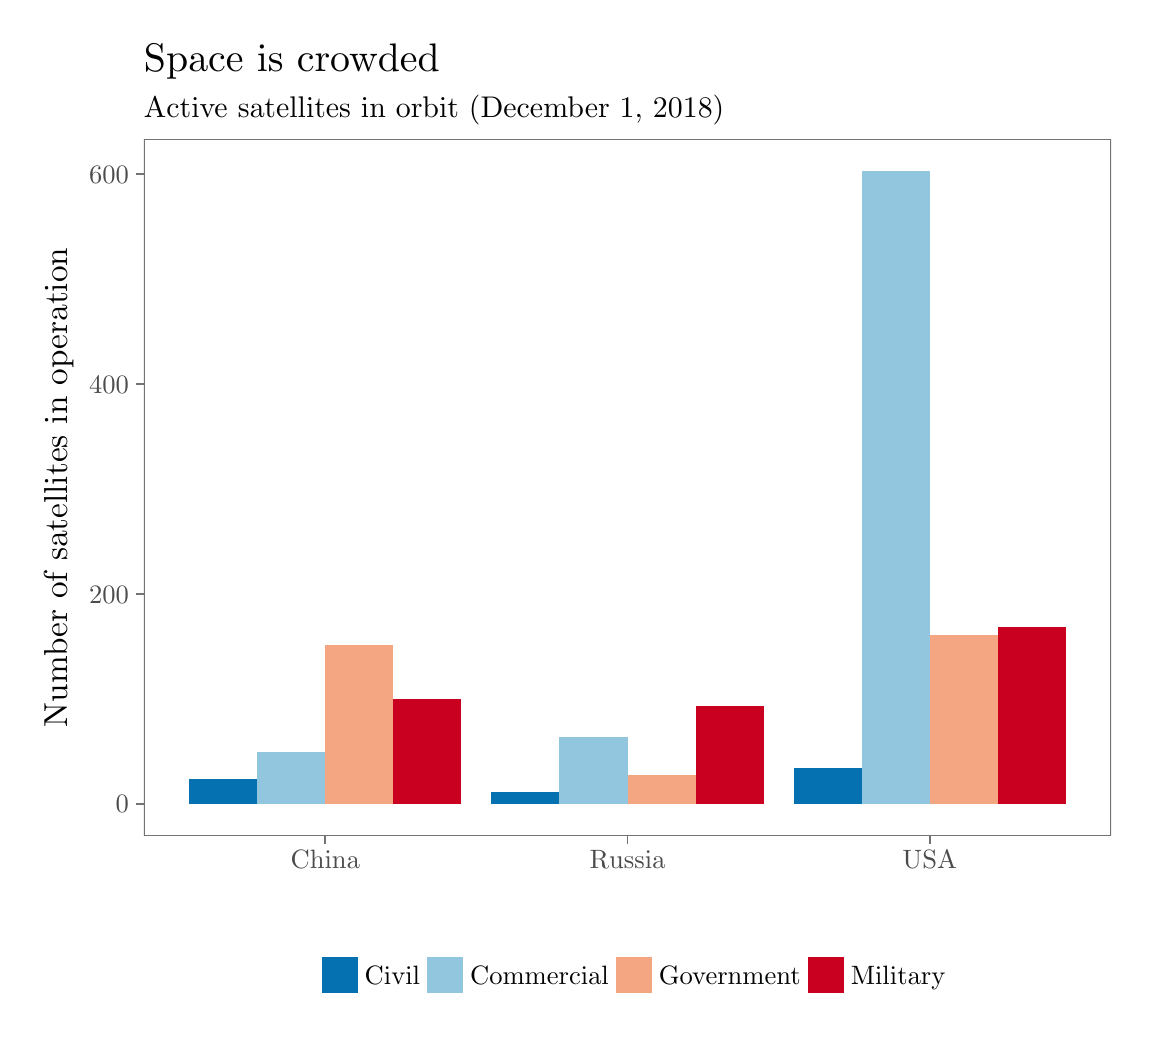
\begin{tikzpicture}[x=1pt,y=1pt]
\definecolor{fillColor}{RGB}{255,255,255}
\path[use as bounding box,fill=fillColor,fill opacity=0.00] (0,0) rectangle (397.48,361.35);
\begin{scope}
\path[clip] (  0.00,  0.00) rectangle (397.48,361.35);
\definecolor{drawColor}{RGB}{255,255,255}
\definecolor{fillColor}{RGB}{255,255,255}

\path[draw=drawColor,line width= 0.6pt,line join=round,line cap=round,fill=fillColor] (  0.00,  0.00) rectangle (397.48,361.35);
\end{scope}
\begin{scope}
\path[clip] ( 42.01, 69.49) rectangle (391.48,320.95);
\definecolor{fillColor}{RGB}{255,255,255}

\path[fill=fillColor] ( 42.01, 69.49) rectangle (391.48,320.95);
\definecolor{fillColor}{RGB}{202,0,32}

\path[fill=fillColor] (132.11, 80.92) rectangle (156.68,118.83);
\definecolor{fillColor}{RGB}{244,165,130}

\path[fill=fillColor] (107.53, 80.92) rectangle (132.11,138.17);
\definecolor{fillColor}{RGB}{146,197,222}

\path[fill=fillColor] ( 82.96, 80.92) rectangle (107.53, 99.50);
\definecolor{fillColor}{RGB}{5,113,176}

\path[fill=fillColor] ( 58.39, 80.92) rectangle ( 82.96, 90.02);
\definecolor{fillColor}{RGB}{202,0,32}

\path[fill=fillColor] (241.32, 80.92) rectangle (265.89,116.18);
\definecolor{fillColor}{RGB}{244,165,130}

\path[fill=fillColor] (216.75, 80.92) rectangle (241.32, 91.16);
\definecolor{fillColor}{RGB}{146,197,222}

\path[fill=fillColor] (192.17, 80.92) rectangle (216.75,105.19);
\definecolor{fillColor}{RGB}{5,113,176}

\path[fill=fillColor] (167.60, 80.92) rectangle (192.17, 85.09);
\definecolor{fillColor}{RGB}{202,0,32}

\path[fill=fillColor] (350.53, 80.92) rectangle (375.10,144.61);
\definecolor{fillColor}{RGB}{244,165,130}

\path[fill=fillColor] (325.96, 80.92) rectangle (350.53,141.96);
\definecolor{fillColor}{RGB}{146,197,222}

\path[fill=fillColor] (301.38, 80.92) rectangle (325.96,309.52);
\definecolor{fillColor}{RGB}{5,113,176}

\path[fill=fillColor] (276.81, 80.92) rectangle (301.38, 93.81);
\definecolor{drawColor}{gray}{0.45}

\path[draw=drawColor,line width= 0.6pt,line join=round,line cap=round] ( 42.01, 69.49) rectangle (391.48,320.95);
\end{scope}
\begin{scope}
\path[clip] (  0.00,  0.00) rectangle (397.48,361.35);
\definecolor{drawColor}{gray}{0.30}

\node[text=drawColor,anchor=base east,inner sep=0pt, outer sep=0pt, scale=  0.96] at ( 36.61, 77.62) {0};

\node[text=drawColor,anchor=base east,inner sep=0pt, outer sep=0pt, scale=  0.96] at ( 36.61,153.44) {200};

\node[text=drawColor,anchor=base east,inner sep=0pt, outer sep=0pt, scale=  0.96] at ( 36.61,229.26) {400};

\node[text=drawColor,anchor=base east,inner sep=0pt, outer sep=0pt, scale=  0.96] at ( 36.61,305.08) {600};
\end{scope}
\begin{scope}
\path[clip] (  0.00,  0.00) rectangle (397.48,361.35);
\definecolor{drawColor}{gray}{0.45}

\path[draw=drawColor,line width= 0.6pt,line join=round] ( 39.01, 80.92) --
	( 42.01, 80.92);

\path[draw=drawColor,line width= 0.6pt,line join=round] ( 39.01,156.74) --
	( 42.01,156.74);

\path[draw=drawColor,line width= 0.6pt,line join=round] ( 39.01,232.56) --
	( 42.01,232.56);

\path[draw=drawColor,line width= 0.6pt,line join=round] ( 39.01,308.38) --
	( 42.01,308.38);
\end{scope}
\begin{scope}
\path[clip] (  0.00,  0.00) rectangle (397.48,361.35);
\definecolor{drawColor}{gray}{0.45}

\path[draw=drawColor,line width= 0.6pt,line join=round] (107.53, 66.49) --
	(107.53, 69.49);

\path[draw=drawColor,line width= 0.6pt,line join=round] (216.75, 66.49) --
	(216.75, 69.49);

\path[draw=drawColor,line width= 0.6pt,line join=round] (325.96, 66.49) --
	(325.96, 69.49);
\end{scope}
\begin{scope}
\path[clip] (  0.00,  0.00) rectangle (397.48,361.35);
\definecolor{drawColor}{gray}{0.30}

\node[text=drawColor,anchor=base,inner sep=0pt, outer sep=0pt, scale=  0.96] at (107.53, 57.48) {China};

\node[text=drawColor,anchor=base,inner sep=0pt, outer sep=0pt, scale=  0.96] at (216.75, 57.48) {Russia};

\node[text=drawColor,anchor=base,inner sep=0pt, outer sep=0pt, scale=  0.96] at (325.96, 57.48) {USA};
\end{scope}
\begin{scope}
\path[clip] (  0.00,  0.00) rectangle (397.48,361.35);
\definecolor{drawColor}{RGB}{1,2,2}

\node[text=drawColor,rotate= 90.00,anchor=base,inner sep=0pt, outer sep=0pt, scale=  1.20] at ( 14.26,195.22) {Number of satellites in operation};
\end{scope}
\begin{scope}
\path[clip] (  0.00,  0.00) rectangle (397.48,361.35);
\definecolor{fillColor}{RGB}{255,255,255}

\path[fill=fillColor] ( 96.23,  6.00) rectangle (337.26, 31.84);
\end{scope}
\begin{scope}
\path[clip] (  0.00,  0.00) rectangle (397.48,361.35);
\definecolor{fillColor}{RGB}{255,255,255}

\path[fill=fillColor] (105.53, 11.69) rectangle (119.99, 26.14);
\end{scope}
\begin{scope}
\path[clip] (  0.00,  0.00) rectangle (397.48,361.35);
\definecolor{fillColor}{RGB}{5,113,176}

\path[fill=fillColor] (106.24, 12.40) rectangle (119.27, 25.43);
\end{scope}
\begin{scope}
\path[clip] (  0.00,  0.00) rectangle (397.48,361.35);
\definecolor{fillColor}{RGB}{255,255,255}

\path[fill=fillColor] (143.59, 11.69) rectangle (158.05, 26.14);
\end{scope}
\begin{scope}
\path[clip] (  0.00,  0.00) rectangle (397.48,361.35);
\definecolor{fillColor}{RGB}{146,197,222}

\path[fill=fillColor] (144.31, 12.40) rectangle (157.34, 25.43);
\end{scope}
\begin{scope}
\path[clip] (  0.00,  0.00) rectangle (397.48,361.35);
\definecolor{fillColor}{RGB}{255,255,255}

\path[fill=fillColor] (211.81, 11.69) rectangle (226.26, 26.14);
\end{scope}
\begin{scope}
\path[clip] (  0.00,  0.00) rectangle (397.48,361.35);
\definecolor{fillColor}{RGB}{244,165,130}

\path[fill=fillColor] (212.52, 12.40) rectangle (225.55, 25.43);
\end{scope}
\begin{scope}
\path[clip] (  0.00,  0.00) rectangle (397.48,361.35);
\definecolor{fillColor}{RGB}{255,255,255}

\path[fill=fillColor] (281.16, 11.69) rectangle (295.61, 26.14);
\end{scope}
\begin{scope}
\path[clip] (  0.00,  0.00) rectangle (397.48,361.35);
\definecolor{fillColor}{RGB}{202,0,32}

\path[fill=fillColor] (281.87, 12.40) rectangle (294.90, 25.43);
\end{scope}
\begin{scope}
\path[clip] (  0.00,  0.00) rectangle (397.48,361.35);
\definecolor{drawColor}{RGB}{1,2,2}

\node[text=drawColor,anchor=base west,inner sep=0pt, outer sep=0pt, scale=  0.96] at (121.79, 15.61) {Civil};
\end{scope}
\begin{scope}
\path[clip] (  0.00,  0.00) rectangle (397.48,361.35);
\definecolor{drawColor}{RGB}{1,2,2}

\node[text=drawColor,anchor=base west,inner sep=0pt, outer sep=0pt, scale=  0.96] at (159.86, 15.61) {Commercial};
\end{scope}
\begin{scope}
\path[clip] (  0.00,  0.00) rectangle (397.48,361.35);
\definecolor{drawColor}{RGB}{1,2,2}

\node[text=drawColor,anchor=base west,inner sep=0pt, outer sep=0pt, scale=  0.96] at (228.07, 15.61) {Government};
\end{scope}
\begin{scope}
\path[clip] (  0.00,  0.00) rectangle (397.48,361.35);
\definecolor{drawColor}{RGB}{1,2,2}

\node[text=drawColor,anchor=base west,inner sep=0pt, outer sep=0pt, scale=  0.96] at (297.42, 15.61) {Military};
\end{scope}
\begin{scope}
\path[clip] (  0.00,  0.00) rectangle (397.48,361.35);
\definecolor{drawColor}{RGB}{1,2,2}

\node[text=drawColor,anchor=base west,inner sep=0pt, outer sep=0pt, scale=  1.08] at ( 42.01,328.85) {Active satellites in orbit (December 1, 2018)};
\end{scope}
\begin{scope}
\path[clip] (  0.00,  0.00) rectangle (397.48,361.35);
\definecolor{drawColor}{RGB}{1,2,2}

\node[text=drawColor,anchor=base west,inner sep=0pt, outer sep=0pt, scale=  1.44] at ( 42.01,345.43) {Space is crowded};
\end{scope}
\end{tikzpicture}

  \label{country_sats}
  \caption{Active satellites, grouped by operating country and purpose}
\end{figure}


\subsection{Threats to the norm against ASATs}
The question of why space has been peacefully militarized but never weaponized is one that this thesis will mostly sidestep. The academic literature on space weaponization was briefly hijacked when Ronald Reagan announced the Strategic Defense Initiative (SDI) on March 23, 1983. Derisively nicknamed ``Star Wars,'' the core promise of the SDI was that, with an Apollo-style research effort, the United States would be able to develop an effective way to end the threat of ballistic nuclear missiles.\footcite{reagan_address_1983} The SDI and the Reagan administration's renewed interest in space conflict overwhelmed the policy research sphere, which was soon consumed with analyzing how best to manage a battlefield that was entirely theoretical, and, to a degree not understood at the time, technologically infeasible. Scholarly work on space policy quickly responded to the possibilities of a world where dueling superpowers were equipped with space-based X-ray lasers, particle beams, and kinetic ballistic missile interceptors---a world which did not exist then, and still belongs to science fiction today.\footcite[p.~1-2]{mowthorpe_militarization_2004}

% Instead, I am concerned with one specific type of space weapon, far more pedestrian than space lasers, but also technologically feasible, successfully tested, virtually unregulated, and potentially catastrophic. A strategic first-strike against American satellites carries the potential to cripple the United States military's intelligence, communications, and ballistics capabilities, to say nothing of the effect on civil society as televisions go dark and cell phones lose signal. Such a strike is made by possible by anti-satellite (ASAT) weapons---and such a strike has remarkably never been executed.

India development things

\section{Conclusion}
\newpage
\printbibliography[heading=subbibliography]

\end{document}
